% =====================================================================
%  Downstream utility of synthetic data for clustering
%  Journal of Classification submission draft
%
%  TEMPLATE
%  --------
%  This compiles against Springer Nature's real sn-jnl.cls (v3.x), which is
%  in this folder together with sn-basic.bst.
%
%  IMPORTANT: sn-jnl.cls here was obtained from a third-party GitHub mirror
%  because Springer's own download page was unreachable from the machine this
%  was built on. Before submitting, replace it with the official copy from
%  Springer's LaTeX author-support page (or open the template on Overleaf and
%  download the zip) and rebuild. The document body should not need changes.
%
%  Journal of Classification is a Math/Physical Sciences title; if their
%  submission guidelines ask for the numbered mathphys style, change the class
%  option to [pdflatex,sn-mathphys-num] and drop sn-mathphys-num.bst in here
%  (it ships with the official zip; the mirror did not carry it).
%
%  \pdfmapfile below is a workaround for a broken font-map index on the build
%  machine. On a normal TeX installation, delete that one line.
% =====================================================================
\documentclass[pdflatex,sn-basic]{sn-jnl}

\pdfmapfile{=local.map}          %% build-machine workaround; delete elsewhere

%%%% Standard Springer Nature preamble (from sn-article.tex)
\usepackage{graphicx}%
\usepackage{multirow}%
\usepackage{amsmath,amssymb,amsfonts}%
\usepackage{amsthm}%
\usepackage{mathrsfs}%
\usepackage[title]{appendix}%
\usepackage{xcolor}%
\usepackage{textcomp}%
\usepackage{manyfoot}%
\usepackage{booktabs}%

\begin{document}

\title{Does Synthetic Data Preserve Cluster Structure?
       A Factorial Evaluation of Partitioning and Hierarchical
       Clustering on {CART}-Generated Data}

\author[1]{Oriol Farr\'es Vilar}
\author[2]{Jordi Cort\'es}
\author[2]{Daniel Fern\'andez}

\affil[1]{Department of Computer Science,
          Universitat Polit\`ecnica de Catalunya, Barcelona, Spain}
\affil[2]{Department of Statistics and Operations Research,
          Universitat Polit\`ecnica de Catalunya, Barcelona, Spain}

\abstract{Synthetic data is increasingly released as a privacy-preserving
substitute for confidential microdata, but its value rests on whether an
analyst reaches the same conclusions from the synthetic release as from the
original records. We evaluate that premise for cluster analysis, a task whose
output depends almost entirely on the geometry of the point cloud and which
therefore probes exactly the higher-order structure that marginal resemblance
checks cannot see. Within a utility-discrepancy framework we compare a
partitioning method ($k$-means) and a hierarchical method (Ward's linkage) on
data generated by sequential CART synthesis, across a factorial design of 144
scenarios crossing the number of groups ($k \in \{2,3,4\}$), separation
($\sigma \in \{0.1,2,6,10\}$), dimensionality ($p \in \{2,5,10\}$), feature
correlation ($\rho \in \{0,0.4\}$) and distribution family (Normal, Gamma),
yielding 72{,}000 synthetic-versus-original evaluations. Separation dominates
recovery of the true number of groups, which rises from $0.27$ in the
overlapping regime to $0.96$ at $\sigma=10$; recovery degrades as $k$ and $p$
grow. The two algorithms are statistically indistinguishable on recovery
($0.585$ versus $0.584$; paired Wilcoxon $p=0.52$; $92\%$ agreement), but they
differ systematically in the geometric bias they impose: $k$-means is the more
conservative estimator on centroid location and dispersion, while its
within-cluster sum-of-squares objective suppresses the size imbalance that
skewed groups would otherwise produce. CART is close to utility-neutral for
spherical Normal components and measurably degrades recovery for skewed Gamma
components, with distortion growing in $p$. We conclude that synthetic-data
utility for clustering is a property of the generator--algorithm--design
triple and must be validated against the intended analysis rather than assumed
from a generic resemblance score.}

\keywords{Synthetic data, Cluster analysis, Statistical disclosure control,
          Analytical utility, Simulation study}

\maketitle

% =====================================================================
\section{Introduction}
% Reviewer note (Jordi, p5): reorganised into the five blocks requested --
% (1) synthetic data, (2) clustering, (3) why synthetic data in clustering,
% (4) the utility concept, (5) objectives, reordered 1-3-2. Subsections
% removed as requested.
% =====================================================================

Synthetic data are artificial records produced by a generative model fitted to
a confidential dataset, released in place of the original records so that the
statistical structure of the data survives while no real individual is
exposed. The idea originates in statistical disclosure control, where
\citet{rubin1993} proposed treating the confidential values as missing and
releasing multiply-imputed replacements, and \citet{little1993} developed the
companion analysis of masked data; \citet{drechsler2011} gives the
book-length treatment of the resulting framework, and \citet{matthews2011}
survey the wider family of disclosure-limitation methods within which
synthesis sits. What began as a mechanism for statistical agencies has since
spread well beyond official statistics, and general-purpose synthesisers are
now distributed as statistical software \citep{nowok2016,templ2017}, with
administrative-data research an active area of application
\citep{kokosi2022}.
Synthetic records are now generated for health services research
\citep{gonzales2023,giuffre2023}, for biobehavioural science, where they also
serve reproducibility and hypothesis generation \citep{quintana2020}, and,
increasingly, through deep generative architectures applied to tabular data
\citep{goyal2024,zhao2024}.

Cluster analysis occupies the opposite end of the analytical pipeline. It is
the canonical unsupervised task: given unlabelled observations, partition them
into groups that are internally homogeneous and mutually distinct. Two
paradigms have dominated applied practice for decades. Centroid-based
partitioning, of which $k$-means \citep{macqueen1967} is the archetype,
minimises the within-cluster sum of squares and remains, by a wide margin, the
most widely deployed clustering algorithm \citep{ahmed2020}. Connectivity-based
agglomeration, typified by Ward's linkage \citep{ward1963}, instead builds a
dendrogram by successive merging and imposes no explicit convexity assumption.
Both remain central to contemporary applications: in single-cell
transcriptomics, where partitions define cell types \citep{zappia2018}, and in
mass cytometry, where the choice among clustering methods materially changes
the biological conclusion \citep{liu2019}.

These two literatures meet whenever a clustering analysis must be performed on
data that cannot be released in raw form. The motivation is partly
privacy---clinical and administrative records are the very datasets on which
subgroup discovery is most valuable and least permissible
\citep{goncalves2020,elemam2020,bhanot2021}---and partly practical, since synthetic
records also serve as an augmentation and model-development resource when
access to the originals is slow or restricted \citep{rankin2020}. In either
case the analyst runs an unsupervised procedure on data they did not observe,
and the question of whether the resulting partition would have been obtained
from the original records is not rhetorical.

That question is the concern of \emph{analytical utility}. It is conventional
to distinguish \emph{general} utility, which asks whether the synthetic data
resemble the original in some global sense, from \emph{specific} utility, which
asks whether a particular analysis yields matching conclusions
\citep{snoke2018}. The distinction matters because the two can come apart: a
generator that reproduces marginal distributions and low-order correlations
faithfully may still distort the higher-order geometry on which a specific
procedure depends. Empirical work bears this out. Benchmarking studies of
synthetic health records find that utility rankings depend heavily on which
downstream task is used to measure them \citep{yan2022,elemam2022}, and direct
replications of published analyses on synthetic counterparts show agreement
that varies by study and by estimand \citep{reinerbenaim2020}. A recent
systematic review of tabular synthesis tools makes the same point from the
measurement side, finding no consensus on which utility metrics should be
reported and little agreement between them \citep{lautrup2024}. Utility is
therefore not a scalar property of a dataset; it is a property of the pairing
between a dataset and the analysis applied to it.

Clustering is a demanding probe of that pairing. Unlike a regression
coefficient, which summarises a conditional mean and is comparatively robust to
local perturbation, a partition is sensitive to the fine structure of the point
cloud: relative positions, local density, separability, within-group
dispersion. Two datasets can share identical means, variances and pairwise
correlations and still yield entirely different partitions. Any distortion a
generator introduces into local geometry should therefore surface in a
clustering analysis before it surfaces in a resemblance check.

This article asks whether CART-based sequential synthesis---the default
non-parametric engine of \texttt{synthpop} \citep{nowok2016}, and the method
most likely to be used in practice on tabular data---preserves the structure
that clustering relies on. It extends the line of inquiry opened by
\citet{chen2025}, which established a simulation harness for this question but
restricted attention to $k$-means on Normal data and relied on a resemblance
statistic that proved insensitive to structural quality. We broaden the scope in
three directions: a second, structurally different clustering paradigm; a
skewed distribution family that exposes the axis-aligned behaviour of
tree-based synthesis; and a battery of ground-truth-referenced structural
metrics that do not depend on the synthetic data alone. Three questions
organise the study.

\begin{description}
\item[RQ1 (Number of groups).] Does CART-synthesised data retain the signal
  needed to recover the true number of clusters, and how does this depend on
  separation, cluster count, dimensionality, correlation and distribution
  family?
\item[RQ2 (Geometry).] Beyond the count, how much geometric
  fidelity---centroid location, within-group dispersion, group balance---is
  lost under synthesis, and which design factors drive that loss?
\item[RQ3 (Algorithm).] Do partitioning and hierarchical methods respond to
  synthetic distortion in the same way, or is one systematically more robust?
\end{description}

% =====================================================================
\section{Methods}
% =====================================================================

The study is a controlled factorial simulation. We first state the two
clustering algorithms, then the generation of reference and synthetic data,
then the metrics used to quantify structural degradation, and finally the way
those metrics are summarised across replications.

\subsection{A discrepancy framework for structural utility}
% Reviewer note (Jordi, p7): old section 2.3 becomes the opening of Methods.

Let $D_R$ denote the reference data and $G$ a generative mechanism, so that
$D_S = G(D_R)$ is the synthetic dataset. Let $A$ be the downstream algorithm,
producing summaries $\theta_R = A(D_R)$ and $\theta_S = A(D_S)$. Utility is
quantified by a discrepancy
\begin{equation}
  \Delta(\theta_R, \theta_S) = f(N, p, \rho, \sigma, k),
  \label{eq:discrepancy}
\end{equation}
studied as a function of the sample size $N$, dimensionality $p$, feature
correlation $\rho$, separation $\sigma$ and number of latent groups $k$. A
generator is useful for a task over a region of design space when $\Delta$
remains small throughout it; the scientific content of an evaluation is the
shape of $\Delta$---which factors inflate it, which leave it unchanged, and
whether different algorithms respond alike.

In the clustering setting, $\theta$ comprises the estimated number of groups
$\hat{k}$ together with the geometry of the recovered partition: its centroids,
its group sizes and its within-group dispersion. Accordingly $\Delta$ is
instantiated as a family of structural-fidelity measures defined in
Section~\ref{sec:metrics}.

To isolate the mechanism we use simulations with known ground truth rather than
real administrative data. Each scenario fixes a configuration
$(N, p, k, \rho, \sigma, \text{distribution})$ for which the true group
membership of every point is known by construction, so recovery is scored
against ground truth rather than against the synthetic data itself. This avoids
the circularity that undermines resemblance-only evaluations, and the factorial
structure allows $\Delta$ in Eq.~\eqref{eq:discrepancy} to be traced as an
explicit function of each design factor.

\subsection{Clustering algorithms}

We compare the two paradigms described in the Introduction because they embody
different geometric assumptions and should therefore respond differently to
the artifacts introduced by tree-based synthesis.

\paragraph{Partitioning ($k$-means).}
$k$-means partitions $N$ observations $\{x_i\}_{i=1}^N$, $x_i \in
\mathbb{R}^p$, into $k$ non-overlapping groups by minimising the within-cluster
sum of squares \citep{macqueen1967}. Writing $\mathcal{C} = \{C_1,\dots,C_k\}$
for the partition and $\mu_j$ for the centroid of $C_j$,
\begin{equation}
  \arg\min_{\mathcal{C}} \sum_{j=1}^{k} \sum_{x_i \in C_j}
    \lVert x_i - \mu_j \rVert^2,
  \qquad
  \mu_j = \frac{1}{|C_j|}\sum_{x_i \in C_j} x_i .
  \label{eq:wcss}
\end{equation}
Lloyd's iteration alternates assignment and update steps until the partition
stabilises; it converges to a local optimum, so we retain the lowest-inertia
solution over ten random initialisations. The method implicitly assumes convex,
isotropic, comparably sized groups, and its decision boundaries are the linear
bisectors of the centroid Voronoi tessellation.

\paragraph{Hierarchical agglomeration (Ward).}
Hierarchical clustering builds a dendrogram by successive merging
\citep{ward1963}. Each observation begins as a singleton; at every step the two
clusters whose merger least increases the total within-cluster error sum of
squares are combined. With
\begin{equation}
  \mathrm{ESS} = \sum_j \sum_{x_i \in C_j} \lVert x_i - \mu_j \rVert^2,
  \qquad
  \Delta_{\text{Ward}}(C_a, C_b)
    = \frac{|C_a|\,|C_b|}{|C_a| + |C_b|}\,
      \lVert \mu_a - \mu_b \rVert^2 ,
  \label{eq:ward}
\end{equation}
a flat partition into $k$ groups is obtained by cutting the dendrogram at the
corresponding height. Ward's linkage makes no explicit convexity assumption and
can follow connected structure, but it is correspondingly more exposed to
spurious local density.

\subsection{Data generation}

\subsubsection{Original data}
% Reviewer note (Jordi, p9): "Reference data" -> "Original data" for
% consistency with the OD/SD notation used throughout; scenarios now in a table.

Each original dataset $D_R$ contains $N = 1000$ observations drawn from a
$k$-component mixture in $\mathbb{R}^p$ with known group labels. Component
centroids are placed so that the minimum pairwise centroid distance equals a
controlled separation $\sigma$: the first centroid sits at the origin and each
subsequent centroid is positioned at distance at least $\sigma$ from those
already placed. Within-component covariance is governed by a correlation matrix
with off-diagonal entries $\rho$, giving spherical components at $\rho = 0$ and
correlated components at $\rho = 0.4$. In the \emph{Normal} family components
are multivariate Gaussian with the specified covariance and centroid. In the
\emph{Gamma} family, skewed components (shape $=1.5$, rate $=5$) are scaled,
given the target correlation through a Cholesky factor, and shifted to the
component centroid, producing curved, right-skewed groups that stress the
axis-aligned nature of CART.

Table~\ref{tab:design} lists the design factors. Each factor is varied to
isolate a distinct hypothesis about when synthesis should succeed or fail:
crossing all five gives $3 \times 4 \times 3 \times 2 \times 2 = 144$
scenarios. Each scenario is replicated across $n = 5$ independent original
datasets, and each original dataset is synthesised $m = 100$ times, so the
executed design comprises $144 \times 5 \times 100 = 72{,}000$
synthetic-versus-original evaluations.

\begin{table}[t]
\centering
\caption{Factors of the simulation design and the question each addresses.
         Crossing all five gives 144 scenarios; with $n=5$ original replicates
         and $m=100$ synthetic draws each, the design yields 72{,}000
         evaluations.}
\label{tab:design}
\small
\begin{tabular}{llp{6.4cm}}
\toprule
Factor & Levels & Rationale \\
\midrule
Separation $\sigma$      & $0.1,\,2,\,6,\,10$ & Spans overlapping to clearly
  distinct groups; tests how much signal must be present before synthesis can
  preserve it. \\
Number of groups $k$     & $2,\,3,\,4$        & More groups means more
  boundaries the generator must reproduce. \\
Dimensionality $p$       & $2,\,5,\,10$       & Each synthesised dimension
  compounds the axis-aligned leaf structure of the generator. \\
Correlation $\rho$       & $0,\,0.4$          & Tests whether dependence
  between features degrades a variable-by-variable synthesis. \\
Distribution family      & Normal, Gamma      & Contrasts smooth spherical
  density with skewed, curved density. \\
\midrule
Sample size $N$          & $1000$ (fixed)     & Held constant so that
  variation is attributable to the factors above. \\
\bottomrule
\end{tabular}
\end{table}

\subsubsection{Synthetic data (CART)}
% Reviewer note (Jordi, p7): old section 2.2 (the synthesis mechanism under
% test) relocated here.

For every original dataset, synthetic data $D_S = G(D_R)$ are generated with
the CART engine of \texttt{synthpop} \citep{nowok2016}, using proper synthesis
and a minimum leaf size of ten. Variables are synthesised sequentially: the
first is sampled from its observed marginal, and each subsequent variable $X_j$
is modelled by a regression tree \citep{breiman1984} on the already-synthesised
variables, with synthetic values drawn from the empirical leaf distribution,
\begin{equation}
  X_j^{\text{syn}} \sim
    \widehat{P}\bigl(X_j \mid
      \text{leaf}(X_1^{\text{syn}},\dots,X_{j-1}^{\text{syn}})\bigr).
  \label{eq:cart}
\end{equation}

This makes the method flexible and distribution-free, but it imposes an
axis-aligned, piecewise-constant structure on the joint distribution: the
synthetic point cloud is assembled from rectangular blocks whose boundaries are
the tree splits. When the original data are smooth and spherical, these blocks
tile the space finely enough to be invisible; when the data are curved, skewed
or heavy-tailed, they become visible as a hardening of smooth density gradients
into discrete steps. Detecting precisely this failure mode, and measuring how
strongly it propagates into the recovered partition, is the purpose of the
evaluation. The ground-truth group label is carried through synthesis so that
the true partition remains available as a reference.

\subsection{Evaluation metrics}
\label{sec:metrics}

Structural utility is quantified by one detection metric and three
geometric-fidelity metrics. The fidelity metrics require the groups recovered
in $D_S$ to be matched to those in $D_R$, since cluster labels are arbitrary.
We build the matrix of pairwise centroid distances between the $k$ original and
$k$ synthetic clusters and solve the resulting linear assignment problem
\citep{kuhn1955}, obtaining the one-to-one matching that minimises total
centroid distance. All fidelity metrics are computed on the aligned clusters.

\paragraph{Recovery of the number of groups.}
For each dataset the number of groups is estimated by maximising the average
silhouette width \citep{rousseeuw1987} over candidates
$\hat{k} \in \{2,\dots,k_{\max}\}$, with $k_{\max} = \min(k+3, 8)$; the
supplementary contingency analysis instead uses a fixed $k_{\max} = 8$ so that
the two data sources are searched over an identical range. A trial succeeds when
$\hat{k} = k$, and for a configuration with $M$ evaluations the recovery rate is
\begin{equation}
  \mathrm{RR} = \frac{1}{M} \sum_{m=1}^{M}
    \mathbb{1}\bigl[\hat{k}_m = k\bigr].
  \label{eq:sr}
\end{equation}
Because $\hat{k}$ is scored against the construction-time ground truth rather
than against the synthetic data, the metric is free of the circularity that
affects resemblance-only evaluations.

\paragraph{Group-balance error ($\Delta G$).}
The Gini coefficient of the cluster-size vector measures how balanced a
partition is. For sizes $\{n_1,\dots,n_k\}$,
\begin{equation}
  G = \frac{\sum_{a=1}^{k}\sum_{b=1}^{k} |n_a - n_b|}
           {2k \sum_{a=1}^{k} n_a},
  \label{eq:gini}
\end{equation}
with $G = 0$ for perfectly equal groups. The fidelity metric is
$\Delta G = |G_S - G_R|$.

\paragraph{Mean centroid distance (MCD).}
With aligned original and synthetic centroids $\mu_j^R$ and $\mu_j^S$,
\begin{equation}
  \mathrm{MCD} = \frac{1}{k} \sum_{j=1}^{k}
    \bigl\lVert \mu_j^R - \mu_j^S \bigr\rVert ,
  \label{eq:mcd}
\end{equation}
so small values indicate that synthesis preserves the location of the group
structure.

\paragraph{Mean variance difference (MVD).}
Writing $v_j^R$ and $v_j^S$ for the mean squared distance of points to their
centroid in aligned original and synthetic clusters,
\begin{equation}
  \mathrm{MVD} = \frac{1}{k} \sum_{j=1}^{k} \bigl| v_j^R - v_j^S \bigr| ,
  \label{eq:mvd}
\end{equation}
capturing whether groups retain their characteristic tightness or spread.

\subsection{Analysis and reporting}
% Reviewer note (Jordi, p10): state explicitly how the metrics are summarised
% across replications, and that visualisation is part of Methods.

All variables are standardised before clustering. Crucially, the scaler is fit
on the original data and applied unchanged to the corresponding synthetic
dataset, so that MCD and MVD are expressed in a common coordinate system;
standardising each dataset separately would rescale away part of the very
distortion the metrics are meant to detect (see Section~\ref{sec:limitations}).

Both the recovery rate and the three geometric-fidelity metrics are computed
over the full design: all 144 scenarios, all five original replicates and all
100 synthetic draws, giving 72{,}000 aligned original--synthetic comparisons.

Results are summarised as follows. Recovery rates are proportions over
evaluations and are reported directly. Fidelity metrics are aggregated first to
a scenario mean and then averaged across scenarios, with dispersion reported as
a $95\%$ interval computed from the scenario-level means; using the scenario as
the unit of replication avoids treating the 100 synthetic draws from one
original dataset as independent. Algorithm comparison uses a paired Wilcoxon
signed-rank test across the 144 scenario-level means.

For visualisation we use the two-dimensional scenarios directly, plotting the
standardised features against each other; no dimensionality reduction is
applied, so the panels show the geometry the algorithms actually operate on. In
the paired original/synthetic displays, cluster labels are matched by the same
Hungarian alignment used for the fidelity metrics and then oriented so that
colour tracks vertical position consistently across panels.

The full design comprises $144$ scenarios, each with five independent original
replicates and $100$ CART draws per replicate, giving $720$ original and
$72{,}000$ synthetic datasets of $N = 1000$ observations. Recovery is evaluated
on all $72{,}000$ original--synthetic pairs. Because estimating the number of
groups requires a silhouette scan over candidate values for each algorithm, and
the geometric metrics require additional fixed-$k$ fits, this amounts to
approximately $10^6$ clustering fits. Every metric reported here is computed on all $72{,}000$ pairs; the
geometric-fidelity metrics additionally require a Hungarian alignment per pair.

Data generation used \texttt{synthpop} \citep{nowok2016} in \textsf{R};
clustering and evaluation used \texttt{scikit-learn} \citep{pedregosa2011} in
Python. Both stages are embarrassingly parallel over scenarios and were
distributed across $18$ worker processes, giving a total runtime of well under
an hour on a single multi-core workstation.

% =====================================================================
\section{Results}
% =====================================================================

\subsection{The block-like artifact}

Figures~\ref{fig:normal} and~\ref{fig:gamma} show a two-dimensional,
two-group scenario at moderate separation ($\sigma = 2$): the original data in
the top row, one CART synthetic replicate below, each partitioned by both
algorithms. Reading across a row shows how the two algorithms divide the same
cloud; reading down a column shows what synthesis did to that division.

On Normal data (Fig.~\ref{fig:normal}) the two compact masses survive
synthesis. The synthetic cloud is visibly sparser in the tails and shows faint
horizontal striping where leaf boundaries fall, but both algorithms cut it in
essentially the same place as they cut the original, and the recovered groups
occupy the same regions. The left column also illustrates why this scenario is
hard for a different reason: at $\sigma = 2$ the true groups overlap
substantially, so neither algorithm reproduces the true labelling exactly---the
boundary they find is a clean vertical split of the combined cloud rather than
the diagonal boundary between the generating components.

On Gamma data (Fig.~\ref{fig:gamma}) the mechanism becomes visible. The
original groups are curved and right-skewed, with a dense corner and long tails
running out along both axes. In the synthetic cloud those smooth tails harden
into discrete, axis-aligned patches, and the dense corner is reproduced as a
set of rectangular blocks rather than a continuous gradient. This is the
signature artifact of sequential tree synthesis: the piecewise-constant leaf
structure of Eq.~\eqref{eq:cart} becomes apparent whenever the underlying
density is not smooth and spherical. The partitions still divide the cloud in
roughly the same orientation, but the boundary is displaced and the resulting
groups have different internal spread---the distortion that the fidelity
metrics quantify below.

\begin{figure}[t]
\centering
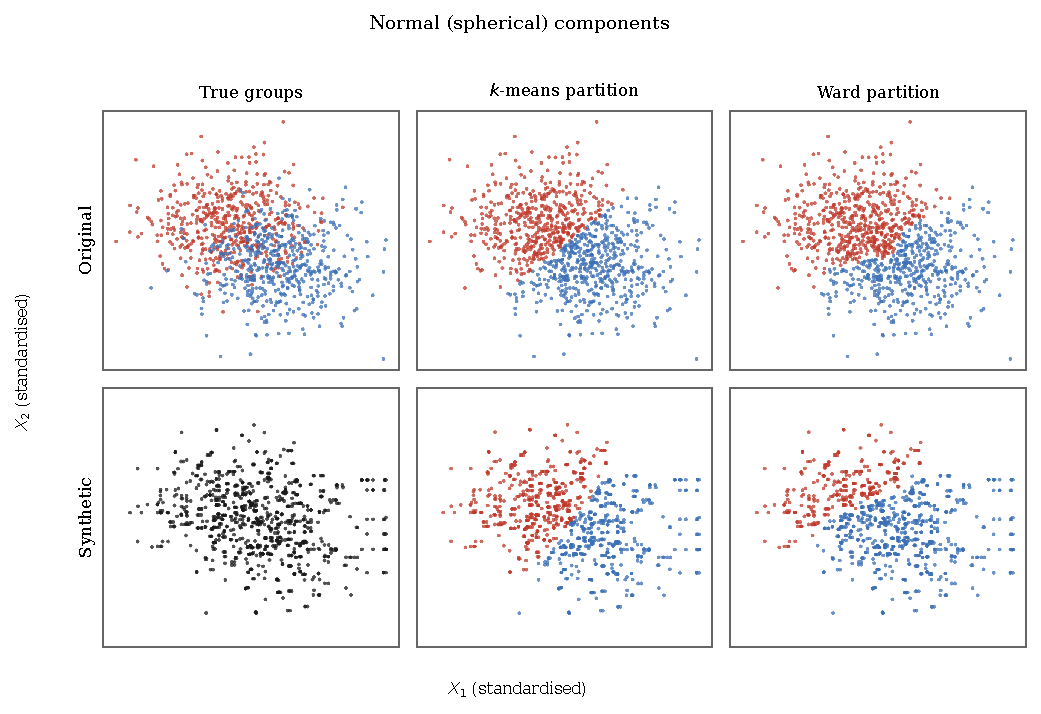
\includegraphics[width=\textwidth]{figures/fig_normal.pdf}
\caption{Normal (spherical) components: geometry largely preserved under
  synthesis. Rows are the original data (top) and one CART synthetic replicate
  (bottom); columns are the true group labels, the $k$-means partition and the
  Ward partition. Colours are matched across rows by Hungarian alignment, so
  the same colour denotes corresponding groups in the original and synthetic
  panels. Scenario: $N = 1000$, $k = 2$, $p = 2$, $\rho = 0$, $\sigma = 2$.}
\label{fig:normal}
\end{figure}

\begin{figure}[t]
\centering
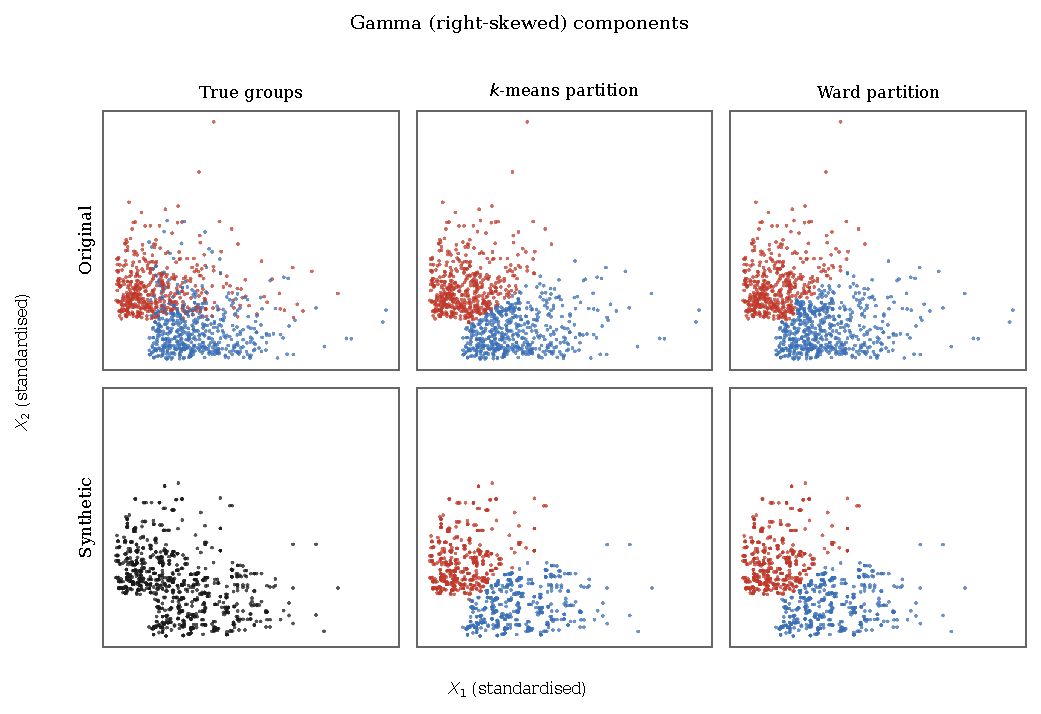
\includegraphics[width=\textwidth]{figures/fig_gamma.pdf}
\caption{Gamma (right-skewed) components: the same synthesis mechanism hardens
  smooth tails into axis-aligned blocks. Panel layout, colour matching and
  scenario as in Fig.~\ref{fig:normal}. Comparing the lower-left panel with the
  upper-left one shows the artifact directly: the continuous density gradient
  of the original becomes a set of discrete rectangular patches.}
\label{fig:gamma}
\end{figure}

\subsection{Number of groups}

Figure~\ref{fig:recovery} shows the recovery rate of Eq.~\eqref{eq:sr} against
separation, stratified by the true number of groups. Two patterns dominate.

Separation is the decisive factor. Averaged over all other factors, recovery
rises from $0.265$ ($k$-means) and $0.289$ (Ward) at $\sigma = 0.1$, through
$0.305$ and $0.301$ at $\sigma = 2$, to $0.812$ and $0.791$ at $\sigma = 6$ and
$0.956$ and $0.954$ at $\sigma = 10$. The transition is sharp: below
$\sigma \approx 2$ recovery is low and dominated by the overlap of the groups
themselves, above $\sigma \approx 6$ it is near-perfect.

Recovery is also far easier for fewer groups. At $k = 2$ the mean recovery rate
is $0.840$ for $k$-means, against $0.476$ at $k = 3$ and $0.437$ at $k = 4$.
The interaction is stark: in the overlapping regime the three- and four-group
cases are almost never recovered, yet the same cases exceed $0.90$ once
$\sigma = 10$. Table~\ref{tab:factors} reports the marginal means for every
design factor. Dimensionality and correlation are secondary, and the
distribution family produces a consistent but modest gap that
Section~\ref{sec:distribution} examines directly.

\begin{figure}[t]
\centering
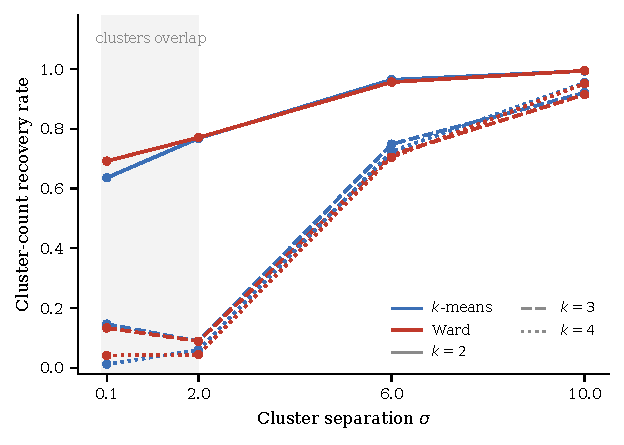
\includegraphics[width=0.62\textwidth]{figures/fig_recovery.pdf}
\caption{Recovery of the true number of groups from CART synthetic data,
  against separation and stratified by the true group count. Recovery is flat
  and low while the groups overlap (shaded) and rises steeply thereafter. The
  two algorithms track each other closely at every $k$.}
\label{fig:recovery}
\end{figure}

\begin{table}[t]
\centering
\caption{Mean recovery rate of the true number of groups by design factor, over
         the full 72{,}000-evaluation design.}
\label{tab:factors}
\small
\begin{tabular}{llrr}
\toprule
Factor & Level & $k$-means & Ward \\
\midrule
Separation $\sigma$ & $0.1$   & 0.265 & 0.289 \\
                    & $2$     & 0.305 & 0.301 \\
                    & $6$     & 0.812 & 0.791 \\
                    & $10$    & 0.956 & 0.954 \\
\addlinespace
Number of groups $k$ & $2$    & 0.840 & 0.853 \\
                     & $3$    & 0.476 & 0.462 \\
                     & $4$    & 0.437 & 0.435 \\
\addlinespace
Dimensionality $p$ & $2$      & 0.619 & 0.623 \\
                   & $5$      & 0.557 & 0.565 \\
                   & $10$     & 0.578 & 0.564 \\
\addlinespace
Correlation $\rho$ & $0$      & 0.569 & 0.575 \\
                   & $0.4$    & 0.600 & 0.593 \\
\addlinespace
Distribution & Normal         & 0.604 & 0.609 \\
             & Gamma          & 0.565 & 0.558 \\
\midrule
Overall & & 0.585 & 0.584 \\
\bottomrule
\end{tabular}
\end{table}

\subsection{Geometric fidelity}

Figure~\ref{fig:fidelity} traces the two geometric-fidelity metrics against
separation. Mean centroid distance falls steeply as groups separate---from
$0.60$ ($k$-means) and $0.86$ (Ward) at $\sigma = 0.1$ to $0.09$ and $0.10$ at
$\sigma = 10$---because well-separated groups pin their centroids robustly
regardless of the local block artifact. Mean variance difference declines in
parallel, from $0.35$ and $0.61$ to $0.11$ and $0.13$. At every separation
level and on both metrics, $k$-means sits below Ward: its centroid averaging
makes it the geometrically more conservative estimator under synthesis. The
intervals overlap at $\sigma \ge 6$, where both methods are close to the floor.

\begin{figure}[t]
\centering
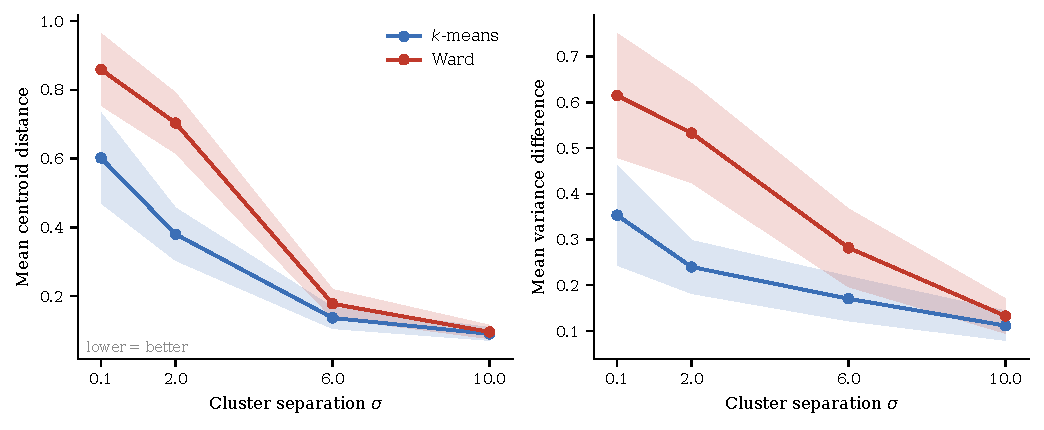
\includegraphics[width=\textwidth]{figures/fig_fidelity.pdf}
\caption{Geometric fidelity against separation. Points are means over the 144
  scenario-level means; bands are $95\%$ intervals computed across scenarios.
  Left: mean centroid distance. Right: mean variance difference. Both decline
  as groups separate, and $k$-means remains below Ward throughout.}
\label{fig:fidelity}
\end{figure}

Dimensionality is the strongest amplifier of variance distortion.
Figure~\ref{fig:balance}(a) shows MVD growing steeply with the number of
variables---for $k$-means from $0.06$ at $p = 2$ to $0.39$ at $p = 10$, and for
Ward from $0.13$ to $0.65$---because each additional synthesised dimension
compounds the axis-aligned leaf structure of Eq.~\eqref{eq:cart}. This is the
mechanism behind the mild degradation of recovery at higher $p$ in
Table~\ref{tab:factors}.

Figure~\ref{fig:balance}(b) shows the group-balance error $\Delta G$ by
distribution family. Both algorithms preserve balance better on Normal than on
Gamma data ($k$-means $0.028$ versus $0.032$; Ward $0.057$ versus $0.065$),
consistent with the block artifact being more disruptive on skewed groups. More
striking is that $k$-means yields systematically lower and tighter $\Delta G$
than Ward at both distributions. This reflects a structural property of the
algorithm rather than better fidelity: the within-cluster sum-of-squares
objective of Eq.~\eqref{eq:wcss} favours partitions of comparable size, so
$k$-means tends to equalise group sizes and thereby suppresses the natural
imbalance that skewed data would otherwise produce. Ward imposes no such
balancing pressure and follows the block-distorted density more literally,
preserving imbalance at the cost of higher variance across replicates. This is
the clearest algorithmic difference the study uncovers---not a difference in
accuracy, but in the kind of geometric bias each method introduces.

\begin{figure}[t]
\centering
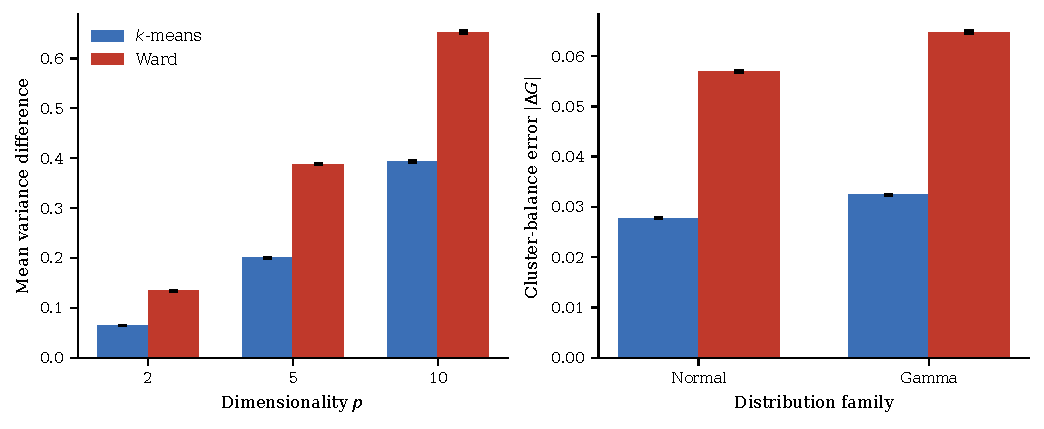
\includegraphics[width=\textwidth]{figures/fig_balance.pdf}
\caption{(a) Mean variance difference by dimensionality: distortion grows
  steeply as dimensions are added, more so for Ward. (b) Group-balance error
  $|\Delta G|$ by distribution family: $k$-means produces lower and tighter
  balance error at both distributions, reflecting the balancing pressure of its
  objective function. Error bars are $95\%$ intervals.}
\label{fig:balance}
\end{figure}

\subsection{Distribution family}
\label{sec:distribution}

The distribution family is the factor that exposes the CART artifact most
directly. Figure~\ref{fig:distribution} stratifies recovery by distribution and
separation. In the overlapping regime the two families are indistinguishable,
because recovery is limited by the overlap rather than by synthesis. In the
informative regime the gap opens: at $\sigma = 6$, $k$-means recovers the
Normal structure $86.2\%$ of the time but the Gamma structure only $76.2\%$
(Ward: $84.4\%$ versus $73.8\%$). By $\sigma = 10$ the gap closes again, as
separation overwhelms the artifact.

This answers RQ1 directly. CART preserves the signal needed to recover the
number of groups well on spherical Normal data, but its hardening of skewed
densities measurably reduces recovery on Gamma data across precisely the range
of separations where recovery is otherwise achievable.

\begin{figure}[t]
\centering
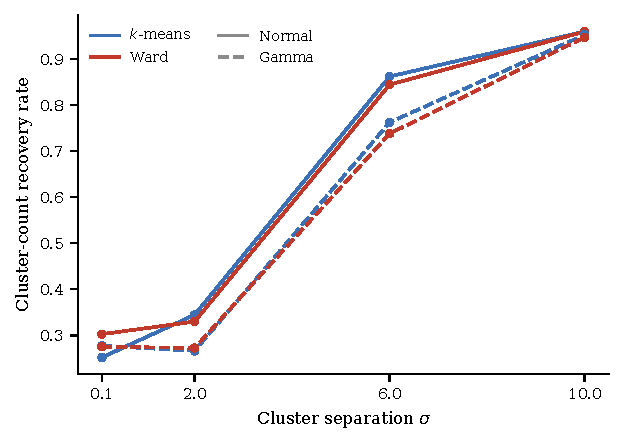
\includegraphics[width=0.62\textwidth]{figures/fig_distribution.pdf}
\caption{Recovery of the number of groups by distribution family and
  separation. The families are indistinguishable while groups overlap and
  diverge in the informative regime, where Gamma data depresses recovery for
  both algorithms.}
\label{fig:distribution}
\end{figure}

\subsection{Agreement between the two algorithms}
% Reviewer note (Jordi, p14): this comparison reads better as the last
% results subsection than as the third.

Whether the two paradigms differ in robustness to synthetic distortion is
RQ3. They do not, at least not on recovery. The overall recovery rates are
$0.585$ ($k$-means) and $0.584$ (Ward); a paired Wilcoxon signed-rank test
across the 144 scenario-level means finds no significant difference
($W = 2838.5$, $p = 0.52$), and the two algorithms agree on the outcome in
$92.1\%$ of individual evaluations. The hypothesis that connectivity-based
clustering would be materially more robust---plausible given its ability to
follow non-convex structure---is not supported.

As a complementary check on internal cohesion, the difference in mean
silhouette width between synthetic and original partitions is small and
centred near zero at every separation. The absolute levels are nearly identical
($k$-means $0.396$ versus $0.397$; Ward $0.376$ versus $0.377$), confirming that
CART neither manufactures nor destroys apparent cluster quality. This is
reassuring, but it also means that silhouette alone would fail to flag the
geometric distortions the other metrics detect---an instructive negative result
for anyone tempted to validate a synthetic release with an internal index.

% =====================================================================
\section{Discussion}
% Reviewer note (Jordi + Dani, p18): "Discussion" rather than "Conclusions".
% =====================================================================

This study evaluated whether CART-generated synthetic data preserves the
structural properties that cluster analysis relies on, comparing $k$-means and
Ward's hierarchical clustering across a 144-scenario factorial design and
72{,}000 synthetic-versus-original evaluations. Four findings emerge.

First, separation dominates recovery of the number of groups. The recovery rate
rises from roughly $0.27$ in the overlapping regime to above $0.95$ at
$\sigma = 10$, with the number of groups the second factor---easy at $k = 2$
($0.84$) and hard at $k \ge 3$ (below $0.48$). Dimensionality, correlation and
distribution family act as secondary modulators. A practical implication is
that a synthetic release is most trustworthy for clustering exactly where
clustering is easiest, and least trustworthy where the analyst most needs help.

Second, the two algorithms are statistically indistinguishable on recovery
($0.585$ versus $0.584$; $p = 0.52$; $92\%$ agreement). Where they differ is in
the geometric bias they introduce. $k$-means is the more conservative
estimator---lower centroid and variance distortion at every separation---and
its objective imposes a balancing bias that suppresses group-size imbalance.
Ward preserves imbalance more faithfully but with higher variance. For an
applied analyst this is the more actionable result than the null on accuracy:
if group sizes are themselves a finding, a $k$-means analysis of synthetic data
will understate imbalance in a way that is invisible from the partition alone.

Third, CART is not utility-neutral, and its failure mode is distributional. On
spherical Normal data it is close to neutral; on skewed Gamma data it hardens
smooth density gradients into axis-aligned blocks, visibly distorting geometry
and measurably depressing recovery in the informative regime. Degradation grows
with dimensionality, as each synthesised dimension compounds the block
structure.

Fourth, and methodologically, an internal validity index is not a sufficient
check. Silhouette geometry is preserved almost exactly even where centroid and
dispersion fidelity degrade substantially. A practitioner who validates a
synthetic release by confirming that its silhouette profile matches the
original will conclude that structure is intact in precisely the settings where
this analysis shows it is not.

An interesting corollary of the design is that clustering can be read in the
other direction, as an instrument rather than an object of study. Because a
partition responds to local density, separability and dispersion
simultaneously, the agreement between partitions recovered from original and
synthetic data functions as a sensitive summary of geometric resemblance---one
that reacts to distortions which marginal and bivariate checks do not see. We
did not pursue this here, but the metrics of Section~\ref{sec:metrics} could be
repurposed as general-utility diagnostics rather than task-specific ones.

\subsection{Relation to previous work}

The study extends \citet{chen2025} in three ways: a structurally distinct
second algorithm, a skewed distribution family that exposes tree-synthesis
artifacts, and ground-truth-referenced structural metrics that do not depend on
the synthetic data alone. The conclusion that CART is a reasonable default for
well-behaved data but degrades on skewed distributions is consistent with the
broader \texttt{synthpop} literature \citep{nowok2016,snoke2018}, and the
qualitative block artifact matches the known axis-aligned bias of sequential
tree synthesis. The finding that utility rankings depend on the downstream task
echoes benchmarking work in the health-records setting
\citep{yan2022,elemam2022}, where the same generator changes position depending
on which analysis is used to score it.

\subsection{Limitations}
\label{sec:limitations}

The evaluation uses controlled simulations with known ground truth rather than
real administrative data. This isolates mechanisms cleanly but limits direct
generalisation to messy data with missingness, mixed types and unknown
data-generating processes. The generator is limited to CART and the algorithms
to $k$-means and Ward; density-based and model-based clustering, and parametric
or deep generative synthesisers, may behave differently. Sample size was fixed
at $N = 1000$, so small-sample behaviour is unexamined, and the
geometric-fidelity metrics were computed on a balanced subset of the synthetic
draws rather than all of them.

Two conventions in the definition of MCD and MVD deserve emphasis, because both
affect the numbers themselves and not only their interpretation. The first is
what the metrics compare. Here they compare the partition recovered from the
original data against the partition recovered from the synthetic data, which is
the quantity a claim about synthesis requires; the superficially similar
practice of comparing a recovered partition against the planted labels of the
same dataset measures clustering accuracy instead, and carries no information
about the generator. The second is scale. Both metrics are computed after
standardising with a scaler fit on the original data and applied unchanged to
the synthetic data, so both are expressed in units of the original feature
scale. Standardising each dataset separately rescales away part of the
distortion the metrics are meant to capture, and omitting standardisation
altogether makes MVD track absolute cluster spread---which grows with $\sigma$
by construction---so that the metric rises with separation when what it is
measuring is the design parameter. Absolute values of MCD and MVD are therefore
not comparable across studies that differ in either convention, and any
replication should state both explicitly.

\subsection{Future work}

The central lesson generalises beyond the specific methods studied: synthetic
data utility is task-relative, and a generator that preserves marginal
resemblance need not preserve the higher-order geometry a clustering workflow
depends on. Practically, the results argue for validating structural
fidelity---distances, dispersion, separability, balance---against the intended
analysis rather than trusting a generic resemblance score. Natural extensions
include other synthesisers (parametric mixtures, copulas, deep generative
models), non-convex and density-based clustering, varying $N$ to probe
small-sample behaviour, and real datasets with established latent structure. A
promising direction is to model the discrepancy $\Delta$ of
Eq.~\eqref{eq:discrepancy} directly as a learned function of the design
factors, turning the utility surface itself into a predictive tool.

Synthetic data generated with CART can reproduce the appearance of clustering
structure while subtly reshaping its geometry. Both algorithms recover
well-separated structure reliably and fail together when groups overlap; where
they diverge is in the bias each imprints on the recovered partition. The
utility of synthetic data for clustering is therefore best understood not as a
property of the data but as a property of the data--generator--algorithm
triple, to be verified rather than assumed.

\bibliography{refs}

\end{document}
